\section{HuMoR Investigation}
\label{sec:humor_investigation}

\subsection{Method}
Our investigation began with a largely qualitative evaluation of the HuMoR model which had two main aims.  First was to stress test the system, to see where it failed, where it succeeded, and if the mentioned benefits in the HuMoR paper \cite{humor} were as described.  The second was to evaluate the model with the defects of the current automated mocap system (described in \chpref{chpt:introduction}) in mind to see if it could complement its functionality, notably if it could improve upon occluded motion, joints flipping and confident but false predictions.

To achieve this goal, a selection of videos were taken containing a variety of motions; fast, slow, abnormal, and with occlusions. The HuMoR system was run on these videos and the results were investigated. The TestOps is performed in 3 stages as described in \secref{sec:humor_test_ops}, where only the 3rd makes use of the HuMoR motion model, we can therefore compare the Stage 2 results to the Stage 3 results to see where the model provided an improvement over a more classical optimisation method.

\subsection{Advantages of HuMoR}
We see a number of situations in which the model shows a clear improvement over stage 2 where the HuMoR model is not used.

In an occluded situation where the 2d pose predictions don't have any information on the legs, the model manages to produce a realistic sitting motion, as shown in \figref{fig:humor_sitting}.

\begin{figure}[!ht]
    \centering
    \subfloat[OpenPose]{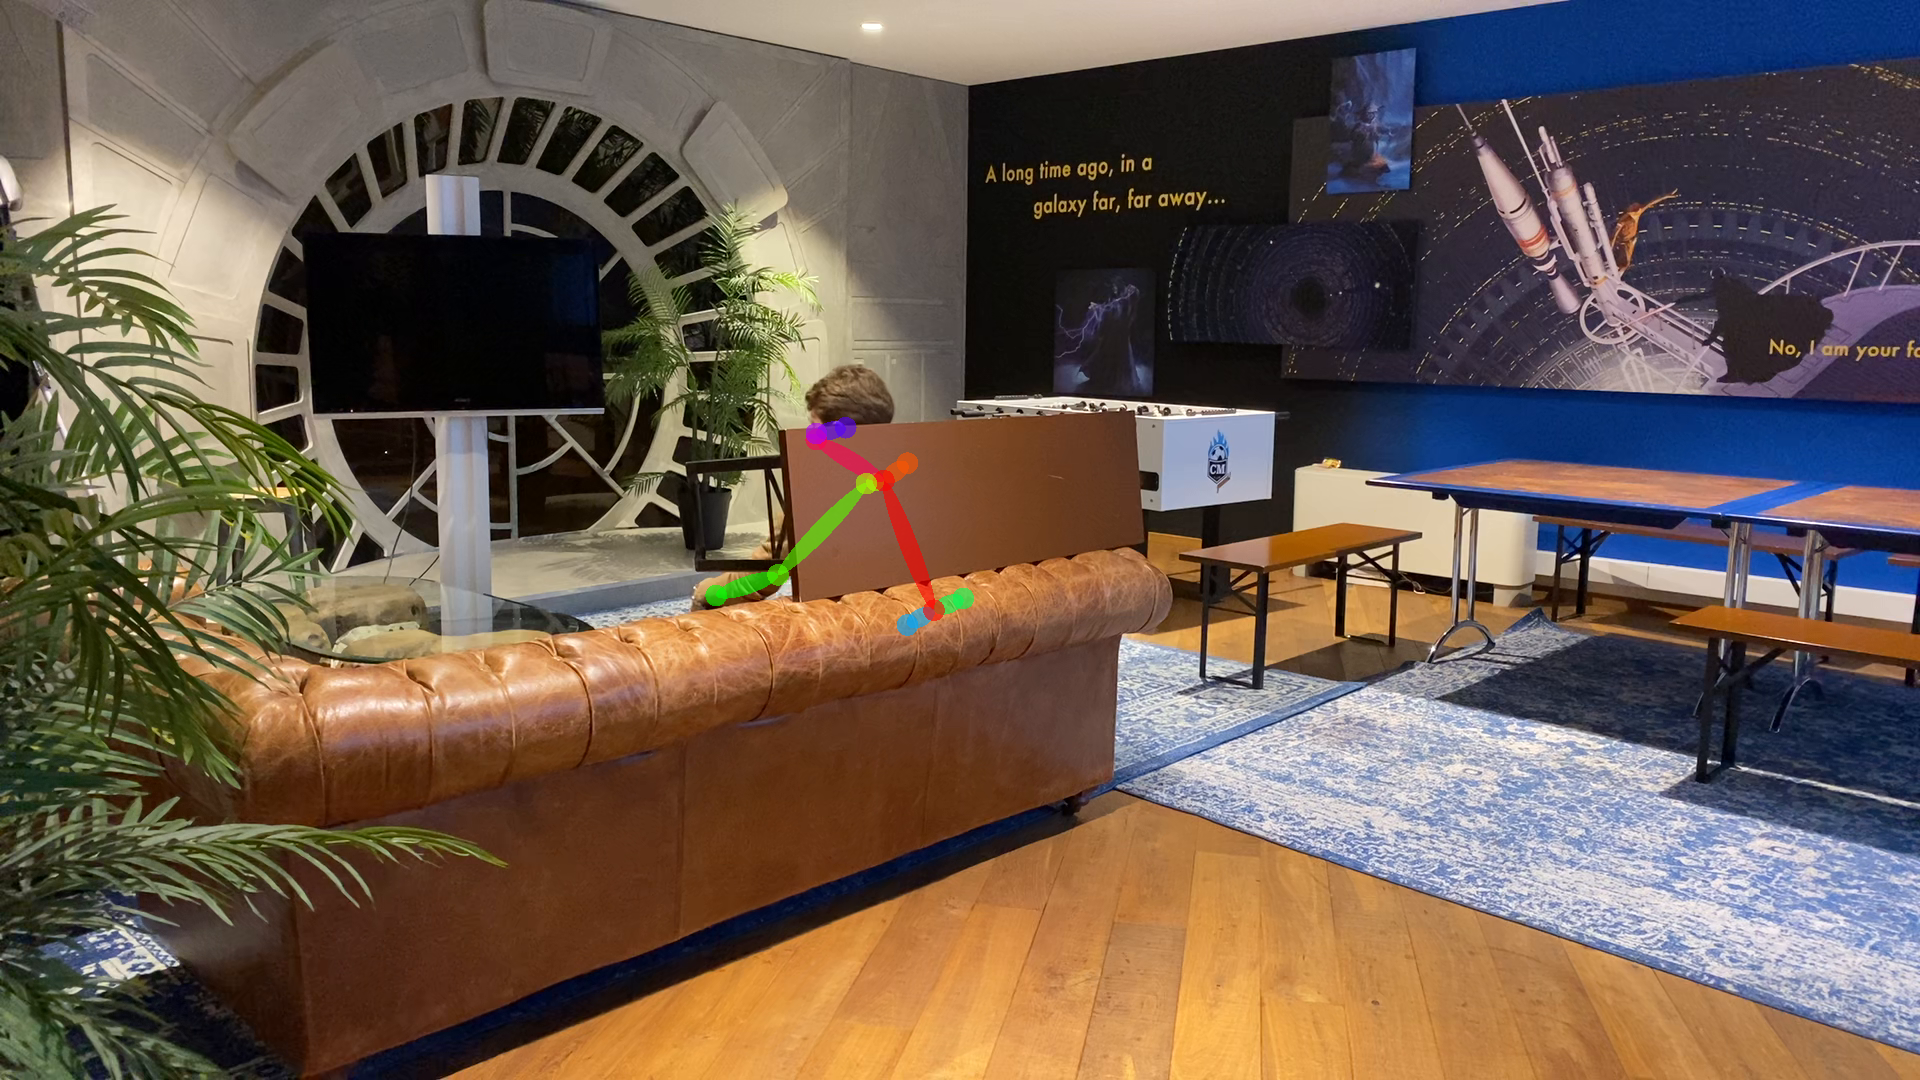
\includegraphics[width=0.3\textwidth]{Figures/humor/qualitative/good/sitting/openPose.png}} 
    \hfil
    \subfloat[Stage 2]{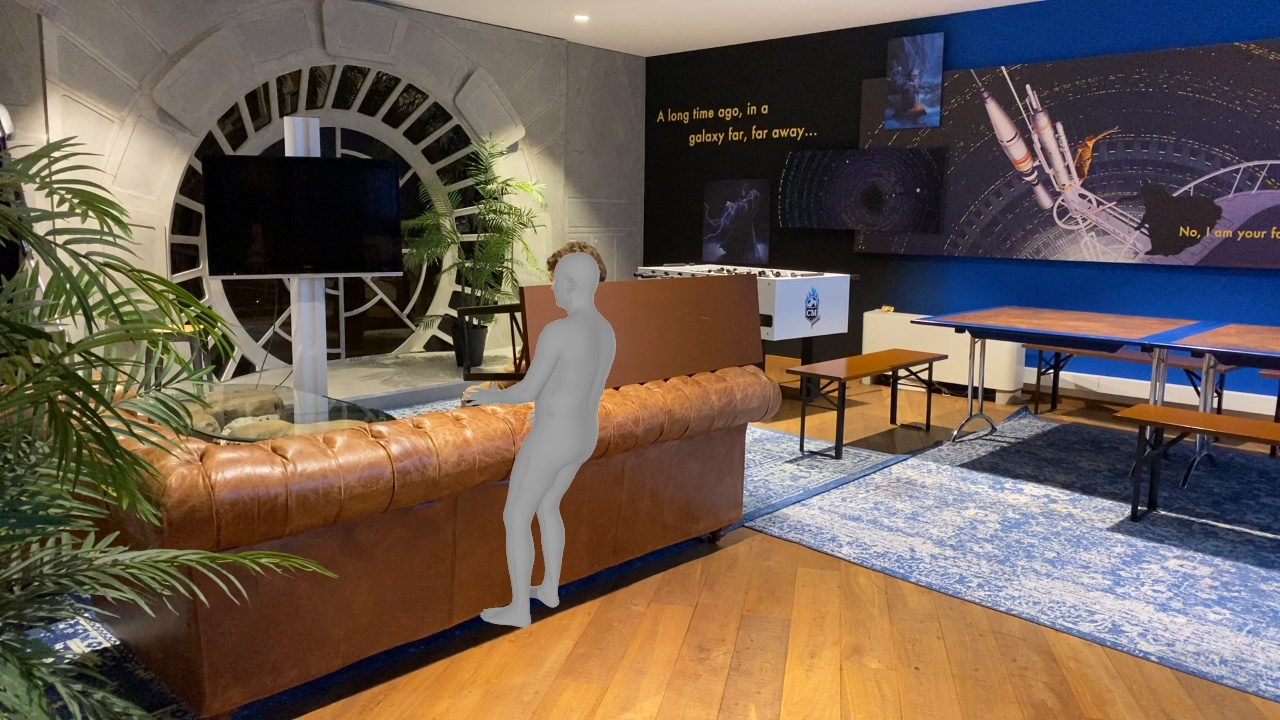
\includegraphics[width=0.3\textwidth]{Figures/humor/qualitative/good/sitting/stage2.jpg}} 
    \hfil
    \subfloat[Stage 3]{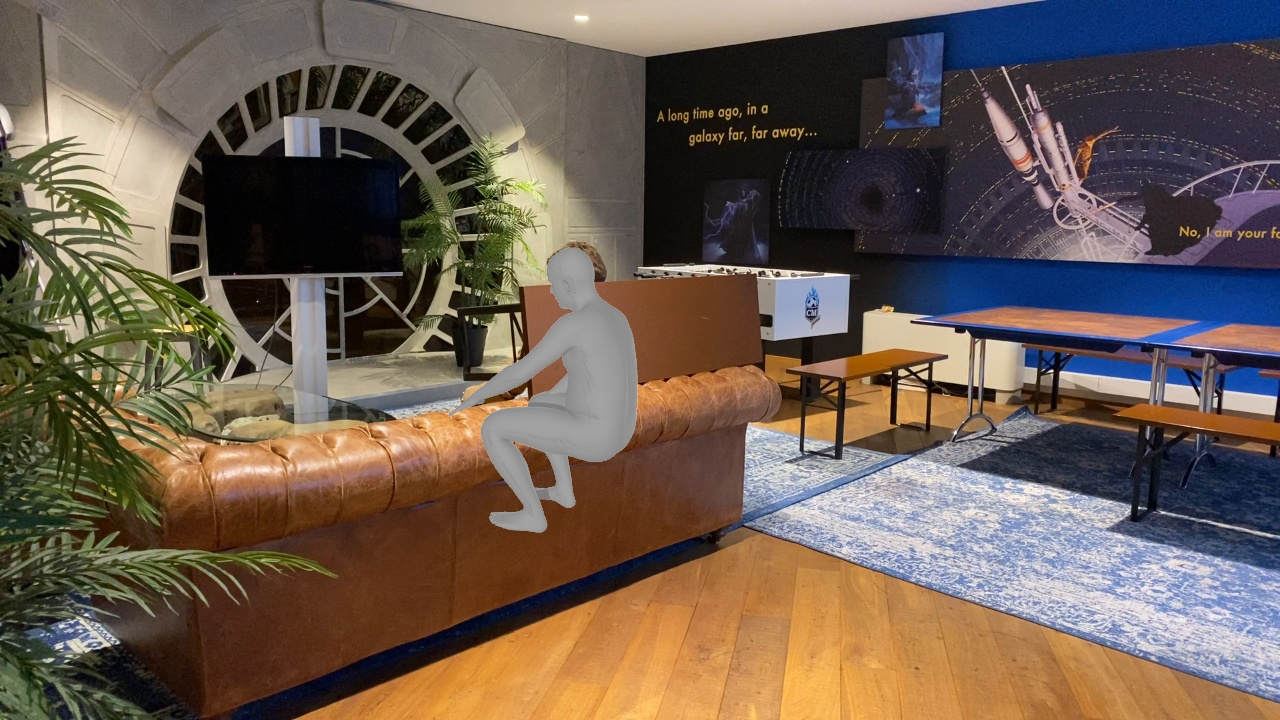
\includegraphics[width=0.3\textwidth]{Figures/humor/qualitative/good/sitting/stage3.jpg}}
    \caption{HuMoR achieving occluded sitting}
    \label{fig:humor_sitting}
\end{figure}

We also note that in many of the less complicated videos HuMoR produces clean motion and deals with many movements without obvious issues. It therefore doesn't seem to regress the easy situations but can improve the more difficult situations, notably occlusions.


\subsection{Drawbacks of HuMoR}

\subsubsection{Occluded walking}
We noted that while HuMoR manages to sit when occluded, it often fails to walk. This seems to be due to the fact that OpenPose \cite{openPose} often predicts both legs on the frames just before the occlusions where only one leg is actually un-occluded, as can be seen in \figref{fig:humor_bad_occluded_walking}. This results in a sequence of poses where the frames before an occlusion indicate that the person is no longer walking, hence making it significantly more difficult for HuMoR to begin walking again during the occlusion. This issue is thus largely due to a dependence on OpenPose and thus on an inheritance of OpenPoses' failure points.

\begin{figure}[!ht]
    \centering
    \subfloat[OpenPose]{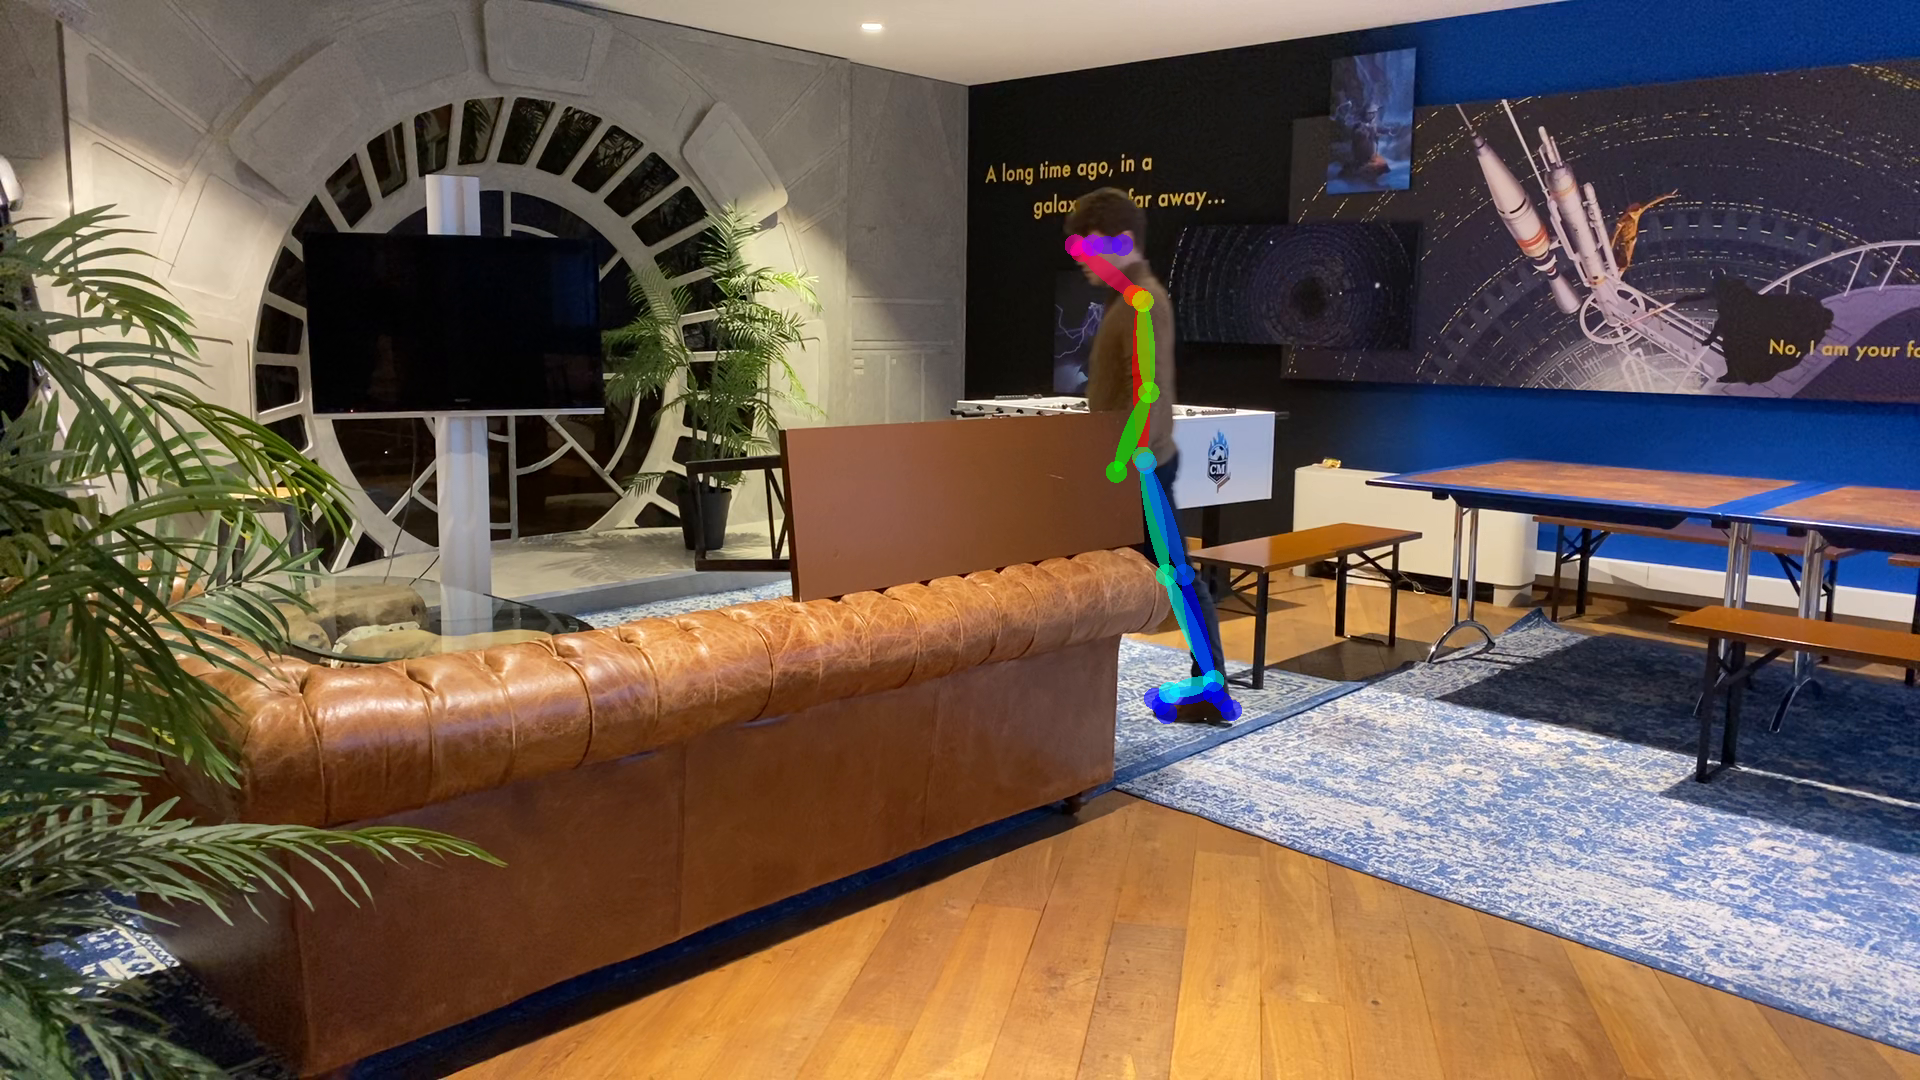
\includegraphics[width=0.2\textwidth]{Figures/humor/qualitative/bad/occluded_walking_failed/openPose.png}} 
    \hfil
    \subfloat[Stage 2]{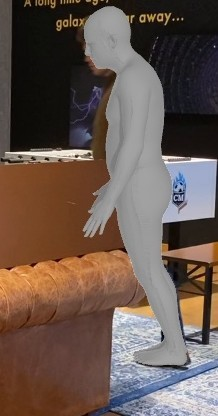
\includegraphics[width=0.2\textwidth]{Figures/humor/qualitative/bad/occluded_walking_failed/stage2.jpg}} 
    \hfil
    \subfloat[Stage 3]{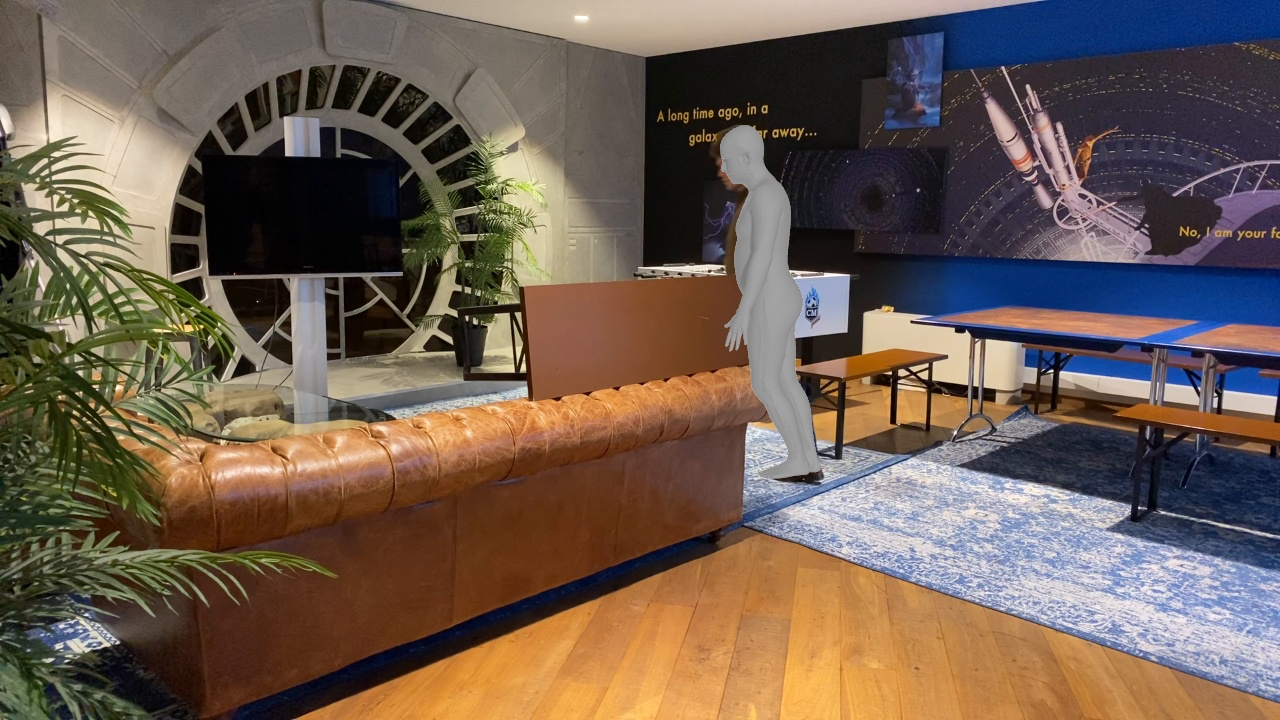
\includegraphics[width=0.2\textwidth]{Figures/humor/qualitative/bad/occluded_walking_failed/stage3.jpg}}
    \caption{Occluded walking failure point, 2 legs predicted instead of 1}
    \label{fig:humor_bad_occluded_walking}
\end{figure}

\subsubsection{Axis-angle representation}
We also found that the choice of axis angle representation for various rotations led to the emergence of commonly known issues that arise from the discontinuities present in the representation \cite{aa_6d_angles}. The shortest path between certain angles in axis angle space enforced by the smoothness regularizer can lead to a 360-degree rotation, as seen in \figref{fig:humor_bad_aa}, among other issues.

\begin{figure}[!ht]
    \centering
    \subfloat[Raw frames]{
        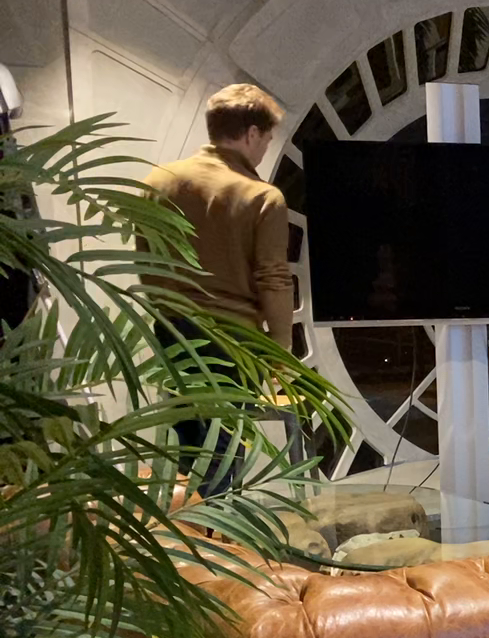
\includegraphics[width=0.2\textwidth]{Figures/humor/qualitative/bad/aa_issue/000329.png}
        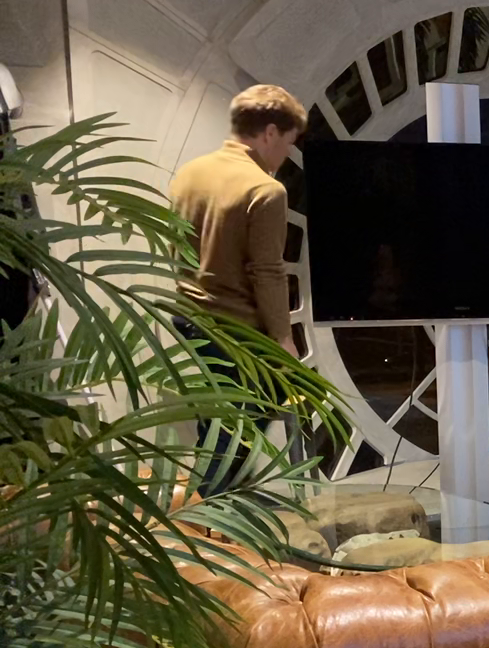
\includegraphics[width=0.2\textwidth]{Figures/humor/qualitative/bad/aa_issue/000335.png}
        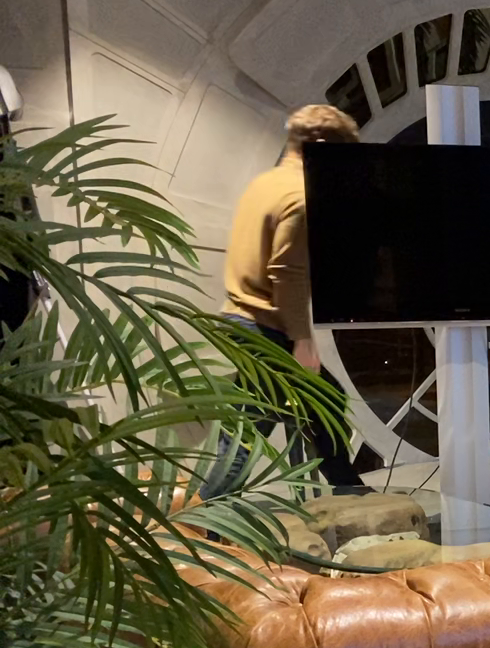
\includegraphics[width=0.2\textwidth]{Figures/humor/qualitative/bad/aa_issue/000343.png}
    } 
    \hfil
    \subfloat[OpenPose]{
        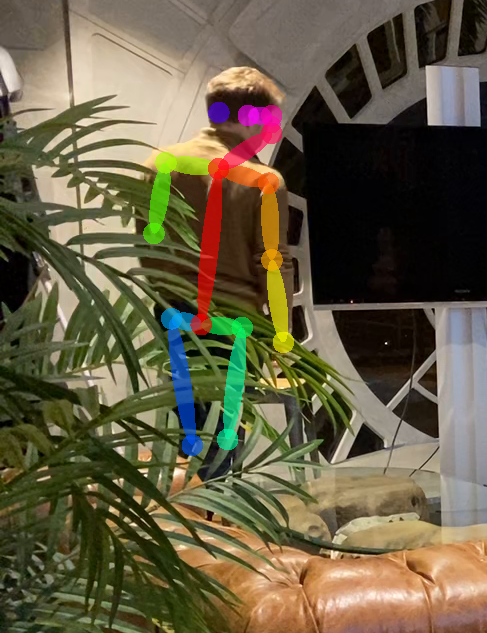
\includegraphics[width=0.2\textwidth]{Figures/humor/qualitative/bad/aa_issue/000329_rendered.png}
        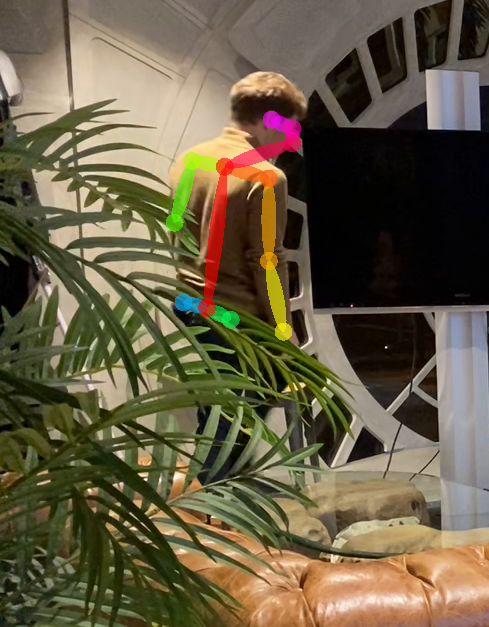
\includegraphics[width=0.2\textwidth]{Figures/humor/qualitative/bad/aa_issue/000335_rendered.png}
        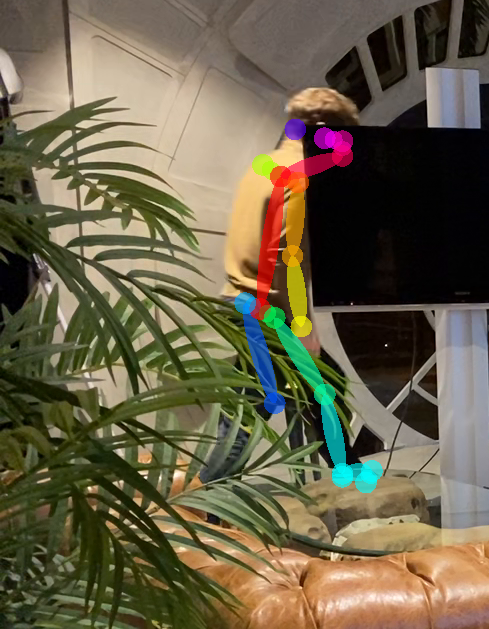
\includegraphics[width=0.2\textwidth]{Figures/humor/qualitative/bad/aa_issue/000343_rendered.png}
    }
    \hfil
    \subfloat[HuMoR, note the full rotation to the left]{
        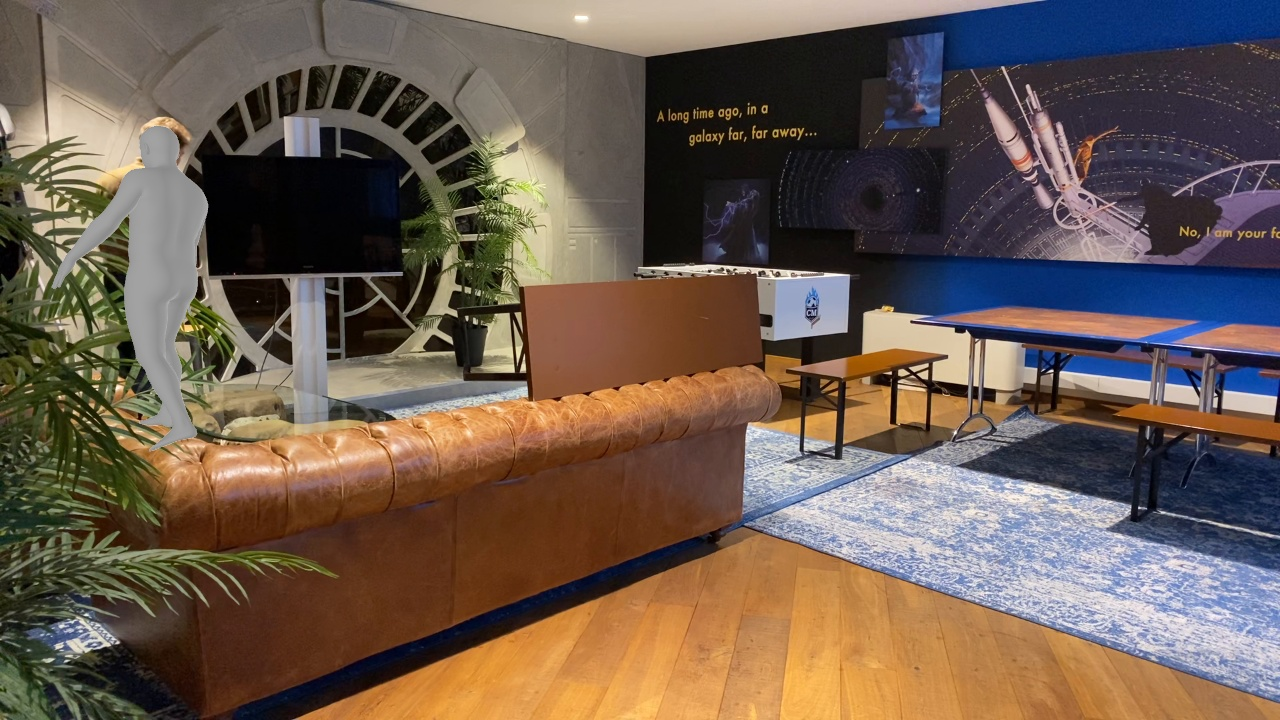
\includegraphics[width=0.2\textwidth]{Figures/humor/qualitative/bad/aa_issue/frame_00000329.jpg}
        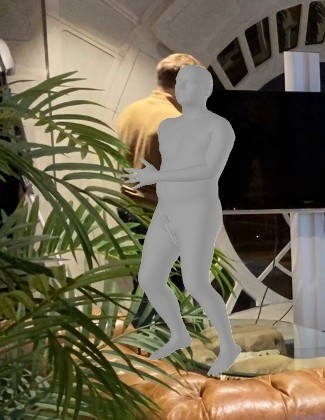
\includegraphics[width=0.2\textwidth]{Figures/humor/qualitative/bad/aa_issue/frame_00000335.jpg}
        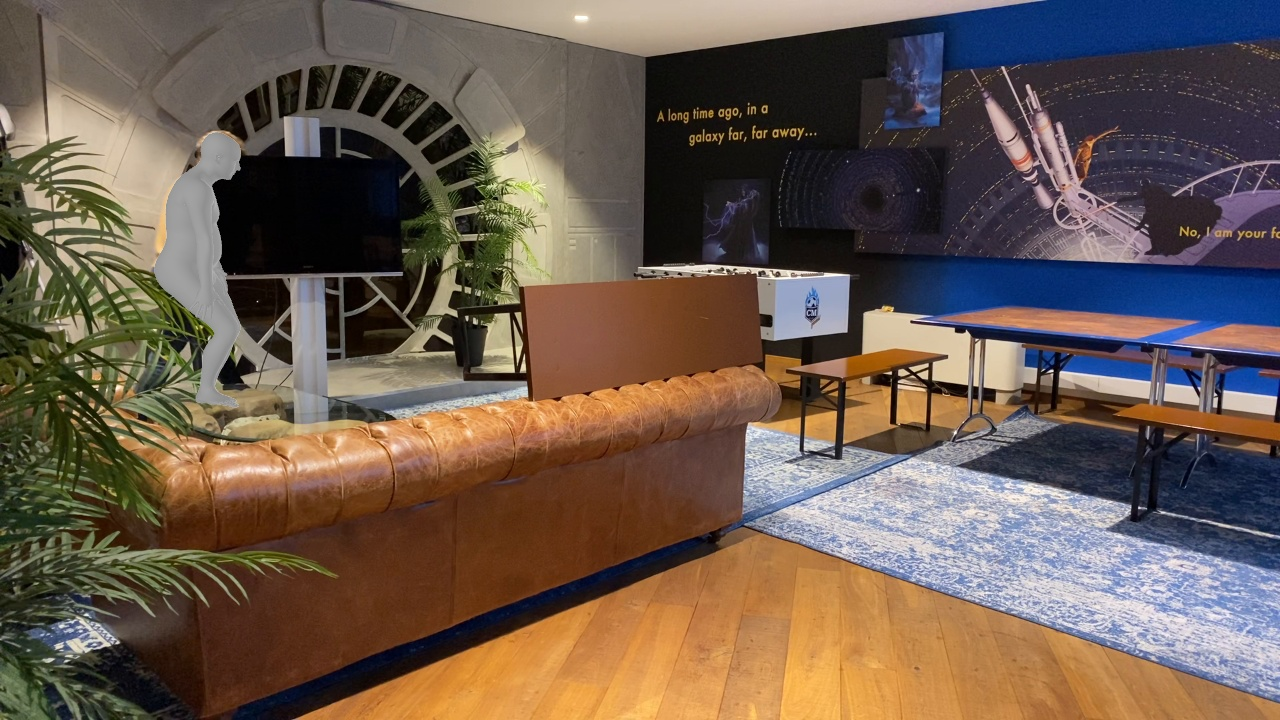
\includegraphics[width=0.2\textwidth]{Figures/humor/qualitative/bad/aa_issue/frame_00000343.jpg}
    }
    \caption{Axis angle issue: dubious rotations}
    \label{fig:humor_bad_aa}
\end{figure}

\subsubsection{Over-smoothed motion}
Next, we saw overly smoothed motion for certain clips, most notably for particularly stylised motions such as dancing.  We also found that if there is a single frame without OpenPose predictions then from that frame onwards the TestOps fails. 

\subsubsection{Autoregressive nature}
We found that the TestOps system would occasionally get itself into a tangle, as seen in \figref{fig:humor_bad_mess}, we assume due to the autoregressive nature resulting in a potentially catastrophic cumulation of errors and found this happened most notably for a sequence containing someone rolling on the floor. It is interesting to note that these sorts of motions were not often, if ever, present in the training data, and so it is likely that the model can fail catastrophically in many more situations, provided that they are sufficiently different from the training data.

\begin{figure}[!ht]
    \centering
    \subfloat[OpenPose]{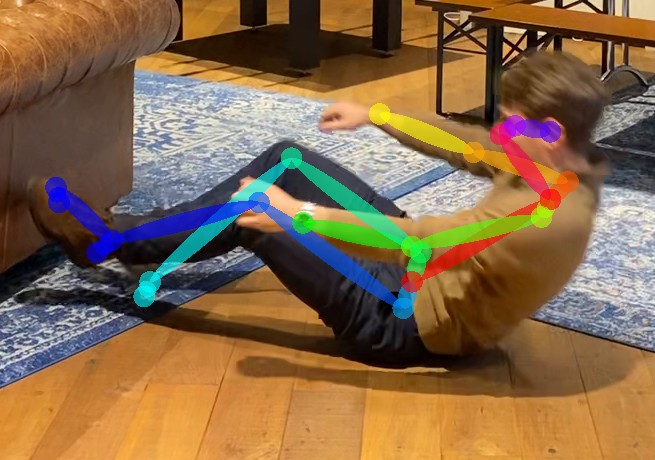
\includegraphics[width=0.3\textwidth]{Figures/humor/qualitative/bad/unrecoverable/openPose.png}} 
    \hfil
    \subfloat[Stage 2]{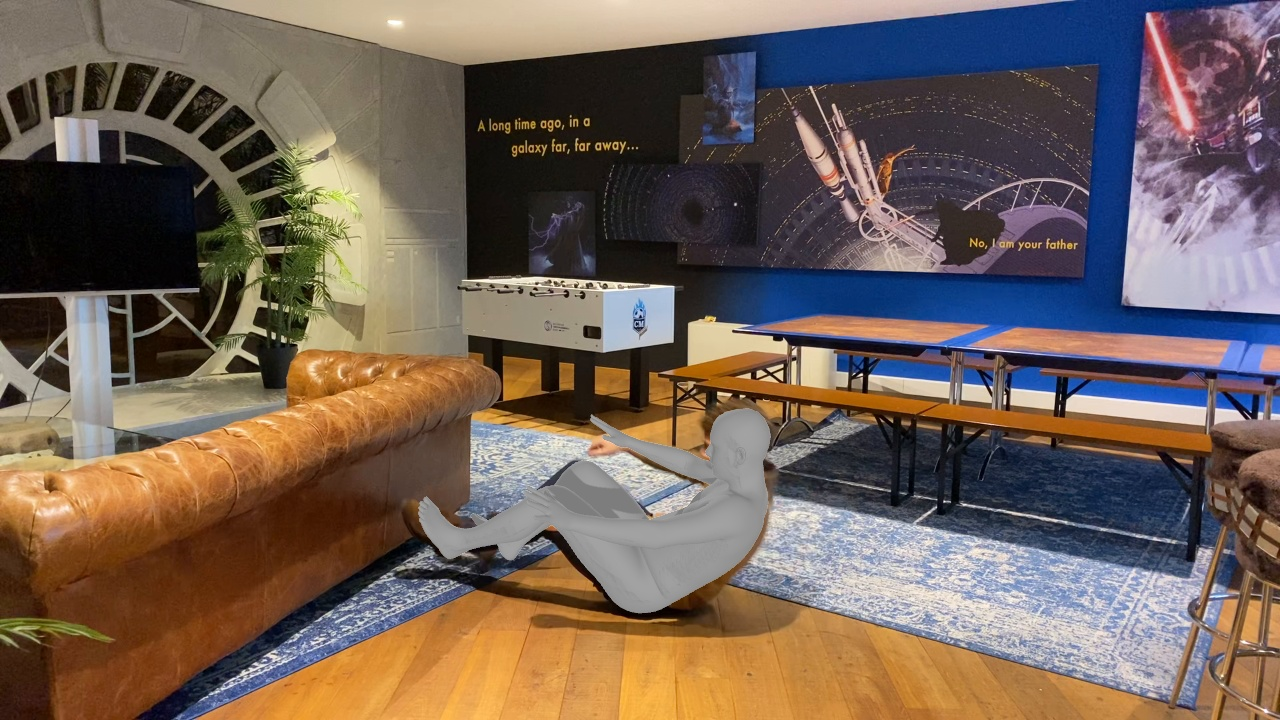
\includegraphics[width=0.3\textwidth]{Figures/humor/qualitative/bad/unrecoverable/stage2.jpg}} 
    \hfil
    \subfloat[Stage 3]{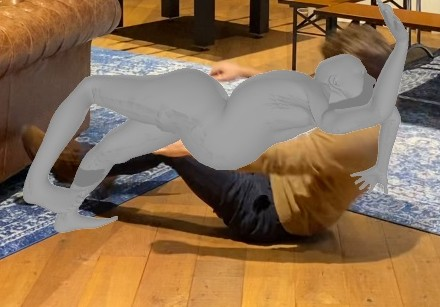
\includegraphics[width=0.3\textwidth]{Figures/humor/qualitative/bad/unrecoverable/stage3.jpg}}
    \caption{HuMoR in a tangle}
    \label{fig:humor_bad_mess}
\end{figure}

Another issue due to the autoregressive nature was the computational burden and high memory usage. The system splits a full video into multiple overlapping subsequences as it is not computationally practical to roll out for the entire sequence. The overlapping sections then have an additional loss applied to them to ensure consistency between the subsequences. While reasonably effective, this demonstrates the heavy computation burden of a long-range autoregression and we find that the shorter the subsequences, the more discontinuities in the optimised motion.

Finally, and most importantly, we found that the TestOps was extremely slow. It took around 20mins per 2s clip, and we could batch at most four 2s clips together, totaling 20mins per 8s on an Nvidia GeoForce 1080ti with 11Gbs memory.

\subsection{Profiling}
To further investigate this speed issue, we profiled the code, as can be seen in \figref{fig:humor_profiling}. We found that the program spent 90\% of its time in the Stage 3 optimiser closure, 56\% of its time performing the backward step and 32\% of its time in the rollout function. Hence it was clear that the speed issue was due to the slow act of rolling out in stage 3 and the large computation necessary to perform the backward step on the enormous computation graph resulting from the rollout.

\begin{figure}[!ht]
    \centering
    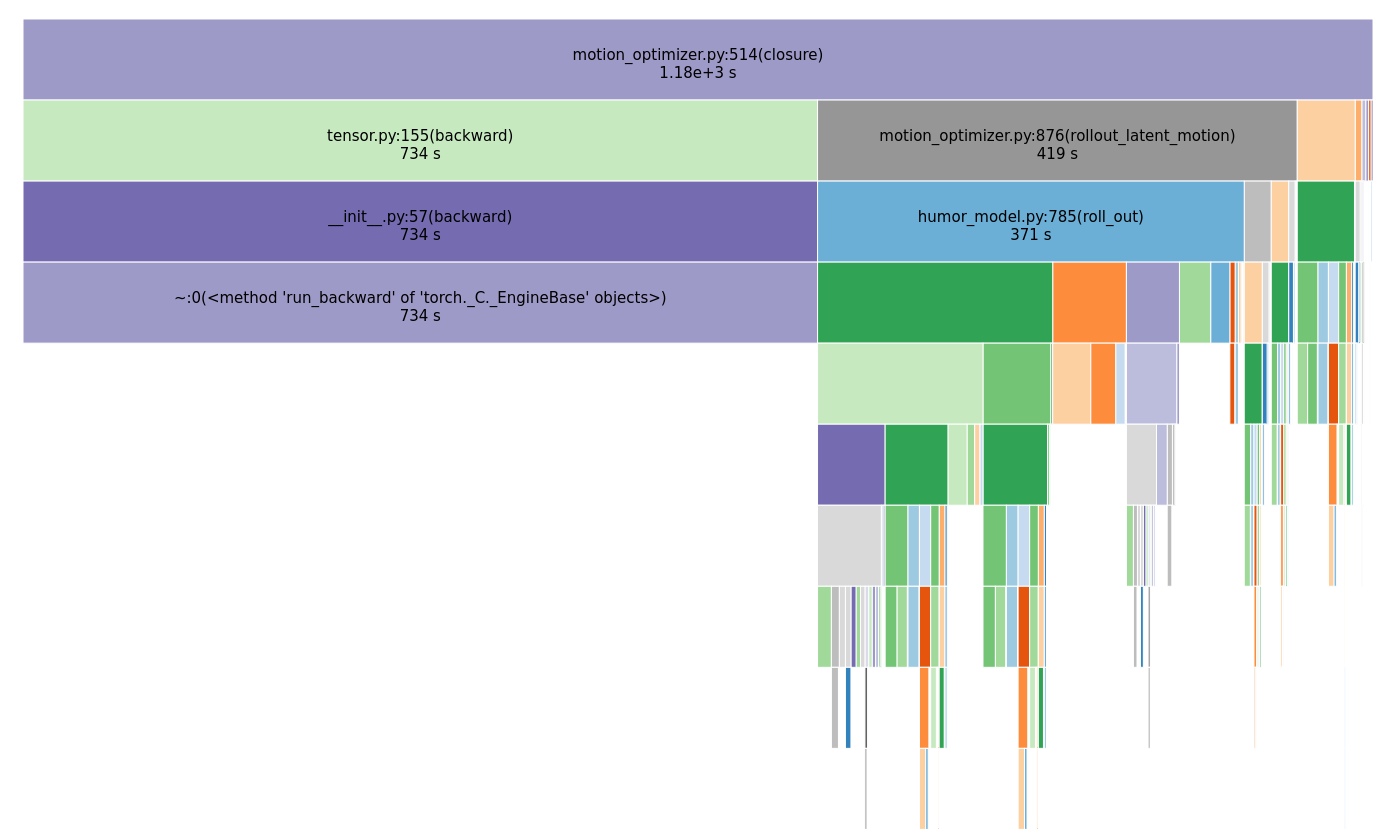
\includegraphics[width=1\textwidth]{Figures/humor/profiling/profiling.png}
    \caption{TestOps profiling}
    \label{fig:humor_profiling}
\end{figure}

\subsection{Investigation Conclusion}
Through this investigation, we found that HuMoR demonstrates a number of positive properties. The model handles occluded sitting motions well and often creates clean and plausible motion. It does however also exhibit numerous issues. The choice of axis angle representation, the dependence on OpenPose, and the smoothed motion all had a good chance of being fixed with different optimiser design choices.  The glaring issue however was the unresonable amount of time the system took, rendering it unusable for our desired goal of having a close to real-time motion capture system. The next step was therefore to speed up the method, and to do so we needed to focus primarily on improving/removing the rollout of the third stage of the optimiser. In the next section, an attempt to do just this is presented.